\documentclass[a4paper]{article}
    \usepackage{minted}
    \usepackage{xcolor}
    \usepackage[colorlinks,linkcolor=black]{hyperref}
    \usepackage[margin=1in]{geometry}
    \usepackage{caption}
    \usepackage{graphicx, subfig}
    \usepackage{float}
    \usepackage{fontspec}
    \setmainfont{Times New Roman}
    \setmonofont{Consolas}
    \definecolor{bg}{rgb}{0.9,0.9,0.9}
    \usemintedstyle{manni}
    \setminted{
    linenos,
    autogobble,
    breaklines,
    breakautoindent,
    bgcolor=bg,
    numberblanklines=false,
    }

\begin{document}
    \tableofcontents
    \newpage
    \section{Problem Description}
        \subsection{Exercise 1}
In the pages of result and author developed in Lab 2, add a paginator which contains two buttons. 
One is for the previous page and the other is for the next page. When these buttons are clicked, some 
Javascript code should be executed to get data from the back-end using AJAX and then replace the current 
page with the data. 
        \subsection{Exercise 2}
In the page of author, add a graph that visualizes the relationship of the author and all collaborators.
In other words, you need to find all the authors who once have cooperated with the author and the cooperations of them. Then, visualize the relationship with Force-Directed Graph. 

Note: the node for the author himself/herself needs to get distinguished from nodes for the collaborators in color. 
        \subsection{Exercise 3(Optional)}
Use one of the classifiers trained in Lab 3 to predict the relationship bewteen any two authors who have ever worked together, and save the relationship into the database. Then, in the visualization graph, mark the nodes for author's students and instructors with different colors.
    \newpage
    \section{Problem Analysis}
        \subsection{Skills Involved}
To implement a paginator, I need to learn and use Javascript and jQuery, a powerful framework of Javascript, in the front-end. And also, in the back-end, I need to write code in PHP. In the meanwhile, some knowledge of HTML, CSS and SQL is required.

To visualize the relationship, the basic usage of D3.js, a Javascript library for visualizing data, is required. And as for the source of data, Python is needed to predict and save the relationship.
        \subsection{Solution Design}
In Lab 2, I have developed two versions of the website: one in raw PHP and one with CodeIgniter. As MVC is useful and makes it easier to organize all the code, I decide to implement all the features based on the website built with CodeIgniter.

To do Exercise 1, my first job is to implement some APIs, which provides the data of search result and authors' papers. After that, modify the pages of result and authors to add the paginator and write some Javascript code.What's more, I can beautify the appearance of the paginator with CSS.

To do Exercise 2 and 3, firstly I will predict and save the relationship. Then just like Exercise 1, APIs are needed to provide data to generate the graph. As for the graph itself, I will just follow the instructions of D3.js to create a Force-Directed Graph.

    \newpage
    \section{Paginator}
        \subsection{Back-end}
Because in this exercise, the job of the back-end is to merely provide data for the front-end, implementing some APIs can be a suitable solution. Therefore, on the basis of Lab 2, I do as follows:
            \subsubsection{API Design}
For the paginator in the page of result, the API looks like these:
\begin{minted}{html}
    {base url}/api/search/{query string}/{page}/{page size}
\end{minted}

And to make it simple to use, \mintinline{html}{{page}} and \mintinline{html}{{page size}} are optional, of which the default values are 1 and 10. So this API can be used in the following ways:
\begin{minted}{html}
    http://localhost/api/search/mike
    http://localhost/api/search/mike/2
    http://localhost/api/search/mike/2/15
\end{minted}

For the paginator in the page of author, the API looks like these:
\begin{minted}{html}
    {base url}/api/papers/{author ID}/{page}/{page size}
\end{minted}
Also,\mintinline{html}{{page}} and \mintinline{html}{{page size}} are optional.

            \subsubsection{Model}
As in Lab 2 I have already implemented \mintinline{html}{Search_result_model} and \mintinline{html}{Author_info_model}, things are relatively easy now: I just need to modify them rather than wirte everything again.

For \mintinline{html}{Search_result_model}, firstly, I add \mintinline{html}{get_result_number()}, a new member function, to the previous model. It takes the query string like "mike" as the parameter and returns how many pieces of result are found. The code is as follows:
\begin{minted}{php}
<?php
    public function get_result_number($authorname="")
    {
        $queryForResultNumber=$this->db->query(
            "SELECT count(*) AS num FROM authors WHERE authorname LIKE '%$authorname%'"
        );
        $result=$queryForResultNumber->result_array();
        return $result[0]["num"];
    }
?>
\end{minted}
Why do I implement this function? Because when turning pages, I need to know how many items there are and then calculate how many pages there are. And this will be further explained in the Controller section.

Beyond that, some minor adjustments are applied to the member function \mintinline{html}{get_search_result()}: adding another two parameters, \mintinline{php}{$begin} and \mintinline{php}{$num}, and modifying its SQL query. And in order to make sure the previous code works fine, these two extra parameters should be optional and suitable by default.
\begin{minted}{php}
<?php
public function get_search_result($authorname="",$begin=0,$num=10)
    {
        $queryForAuthor=$this->db->query(
            "... LIMIT $begin,$num;"
        );
        //unmodified and thus omitted
    }
?>
\end{minted}

For \mintinline{html}{Author_info_model}, more complicated but roughly similar modifications are made. Firstly, also implement a function to get the number of papers as follows: (Note that it returns an array rather than merely a value)
\begin{minted}{php}
<?php
    public function get_paper_number($authorID=NULL)
    {
        if(!$authorID)
            return NULL;
        else{
            $queryForPaperNum=$this->db->query(
                "SELECT COUNT(*) AS num FROM paper_author_affiliation WHERE authorid='$authorID';");
            $queryForCitedPaperNum=$this->db->query(
                "SELECT COUNT(DISTINCT paper_author_affiliation.paperid) AS num
                FROM paper_author_affiliation,paper_reference 
                WHERE paper_author_affiliation.authorid='$authorID' 
                    AND 
                paper_author_affiliation.paperid = paper_reference.referenceid;"
                );
            $queryForUncitedPaperNum=$this->db->query(
                "SELECT COUNT(*) AS num FROM paper_author_affiliation 
                WHERE paper_author_affiliation.authorid='$authorID' 
                    AND 
                    ( SELECT count(1) FROM paper_reference 
                        WHERE paper_reference.referenceid 
                            = paper_author_affiliation.paperid
                    ) = 0;"
                );
            $result=array();
            $result["cited"]=$queryForCitedPaperNum->row_array()["num"];    
            $result["uncited"]=$queryForUncitedPaperNum->row_array()["num"];
            $result["all"]=$queryForPaperNum->row_array()["num"];
            return $result;
        }
    }
?>
\end{minted}
Then, I need to adjust the previous function \mintinline{html}{get_author_info()} to get papers in different pages. 

But there is an critical issue : for cited papers and uncited papers, my SQL queries are distinct. 

To solve this issue, as you might have guessed from the function \mintinline{html}{get_paper_number()}, I compare the position of target papers with the number of cited papers and uncited papers to decide how many cited papers and how many uncited papers should be return. In the following code, I omit some unimportant code and the definition of two functions: \mintinline{html}{get_cited_papers()} and \mintinline{html}{get_uncited_papers()} is also skipped for conciseness.
\begin{minted}{php}
<?php
    public function get_author_info($authorID=NULL,$begin=0,$num=10,$paperNum=NULL)
    {
        //omitted
        $papers=array();
        if($begin>=0 and $begin+$num<=$paperNum["cited"]){
            foreach ($this->get_cited_papers($authorID,$begin,$num) as $row) {
                array_push($papers, $this->handle_one_paper($row));
            }
        }else if($begin<=$paperNum["cited"]-1 and $begin+$num-1>=$paperNum["cited"]){
            $paperCnt=0;
            foreach ($this->get_cited_papers($authorID,$begin,$num) as $row) {
                $paperCnt+=1;
                array_push($papers, $this->handle_one_paper($row));
            }
            $newNum= $num-$paperCnt;
            foreach ($this->get_uncited_papers($authorID,0,$newNum) as $row) {
                $row["citation"]=0;
                array_push($papers, $this->handle_one_paper($row));
            }            
        }else if($begin>=$paperNum["cited"]){
            $newBegin=$begin-$paperNum["cited"];
            foreach ($this->get_uncited_papers($authorID,$newBegin,$num) as $row) {
                $row["citation"]=0;
                array_push($papers, $this->handle_one_paper($row));
            }
        }
        $result["papers"]=$papers;
        return $result;
    }
?>
\end{minted}
            \subsubsection{View}
Just as the usual practice, my APIs return JSON encoded data. So the part of view is quite simple and easy to understand:
\begin{minted}{php}
<?php 
    echo json_encode($json);
 ?>
\end{minted}
            \subsubsection{Controller} 
Though in Lab 2 there's already a controller named Page, I decide to create a new controller as what I'm going to do in this exercise is rather different from that in Lab 2. The new controller is called \mintinline{html}{API}.
\begin{minted}{php}
<?php 
class API extends CI_Controller{

    public function __construct()
    {
        parent::__construct();
        $this->load->model('Search_result_model');
        $this->load->model('Author_info_model');
    }
}
?>    
\end{minted}
Then, to handle URLs like \mintinline{php}{/api/search/mike/2/10}, the controller needs a member function named \mintinline{php}{search()}. 
\begin{minted}{php}
<?php
public function search($query=NULL,$page=1,$pageSize=10)
    {
        $json=array();
        $data=array();
        if(!$query){
            $json["success"]=0;
            $json["reason"]="The query is NULL.";
        }else{
            $resultNum=$this->Search_result_model->get_result_number($query);
            if($resultNum==0){
                $json["success"]=0;
                $json["reason"]="No result found.";
            }else{
                $maxPage=(int)(($resultNum-1)/$pageSize) + 1;
                if($page>$maxPage){
                    $json["success"]=0;
                    $json["reason"]="Out of page limit.";
                    $json["resultNum"]=$resultNum;
                    $json["pageSize"]=$pageSize;
                    $json["maxPage"]=$maxPage;
                    $json["page"]=$page;
                    $json["itemNum"]=0;
                }else{
                    $json["success"]=1;
                    $json["resultNum"]=$resultNum;
                    $json["pageSize"]=$pageSize;
                    $json["maxPage"]=$maxPage;
                    $json["page"]=$page;
                    $begin=$pageSize*($page-1);
                    $json["searchResult"] = 
                        $this->Search_result_model ->get_search_result($query,$begin,$pageSize);
                    $json["itemNum"]=count($json["searchResult"]);
                }
            }
        }
        $data["json"]=$json;
        $this->load->view("templates/json.php",$data);
    }
?>
\end{minted}
To handle URLs like \mintinline{php}{/api/papers/7F960928/2/9}, a function named \mintinline{php}{papers()} is developed.
\begin{minted}{php}
<?php
    public function papers($ID=NULL,$page=1,$pageSize=10)
    {
        $json=array();
        $data=array();
        if(!$ID){
            $json["success"]=0;
            $json["reason"]="Please specify the ID.";
        }else{
            $paperNum=$this->Author_info_model->get_paper_number($ID);
            if($paperNum["all"]==0){
                $json["success"]=0;
                $json["reason"]="No paper found!";
            }else{
                $maxPage=(int)(($paperNum["all"]-1)/$pageSize)+1;
                if($page>$maxPage){
                    $json["success"]=0;
                    $json["paperNum"]=$paperNum;
                    $json["pageSize"]=$pageSize;
                    $json["maxPage"]=$maxPage;
                    $json["page"]=$page;
                    $json["reason"]="Out of page limit!";
                }else{
                    $json["success"]=1;
                    $json["paperNum"]=$paperNum;
                    $json["pageSize"]=$pageSize;
                    $json["maxPage"]=$maxPage;
                    $json["page"]=$page;
                    $begin=$pageSize*($page-1);
                    $json["papers"]=$this ->Author_info_model ->get_author_info(
                        $ID,$begin,$pageSize,$paperNum)["papers"];
                    $json["itemNum"]=count($json["papers"]);
                }
            }
        }
        $data["json"]=$json;
        $this->load->view("templates/json.php",$data);
    }
?>
\end{minted}
So far, the part of back-end has been completed.

If you visit \mintinline{html}{/api/search/mike/1/3}, you will get JSON data like this:
\begin{minted}{json}
{
    "success": 1,
    "resultNum": "96",
    "pageSize": "3",
    "maxPage": 32,
    "page": "1",
    "searchResult": [
        {
            "authorID": "7A49F117",
            "authorName": "Mike Dahlin",
            "paperNum": "8",
            "affiliationID": "05282E0D",
            "affiliationName": "University Of Texas At Austin"
        },
        {
            "authorID": "7923B504",
            "authorName": "Mike Perkowitz",
            "paperNum": "8",
            "affiliationID": "0C01DCFD",
            "affiliationName": "University Of Washington"
        },
        {
            "authorID": "7FC83BF2",
            "authorName": "Mikel Rodriguez",
            "paperNum": "7",
            "affiliationID": "01C3C549",
            "affiliationName": "Ecole Normale Superieure"
        }
    ],
    "itemNum": 3
}
\end{minted}
If you visit \mintinline{html}{/api/papers/7F960928/1/2}, you will get JSON data like this:
\begin{minted}{json}
{
    "success": 1,
    "paperNum": {
        "cited": "119",
        "uncited": "36",
        "all": "155"
    },
    "pageSize": "2",
    "maxPage": 78,
    "page": "1",
    "papers": [
        {
            "paperID": "7E4B8249",
            "paperTitle": "An Iterative Image Registration Technique With An Application To Stereo Vision",
            "paperPublishYear": "1981",
            "conferenceID": "47C39427",
            "conferenceName": "IJCAI",
            "citation": "414",
            "authors": [
                {
                    "subAuthorName": "Bruce D Lucas",
                    "subAuthorID": "7EEBF5D3",
                    "subAuthorSequence": "1"
                },
                {
                    "subAuthorName": "Takeo Kanade",
                    "subAuthorID": "7F960928",
                    "subAuthorSequence": "2"
                }
            ]
        },
        {
            "paperID": "807A8028",
            "paperTitle": "A Statistical Method For 3d Object Detection Applied To Faces And Cars",
            "paperPublishYear": "2000",
            "conferenceID": "45083D2F",
            "conferenceName": "CVPR",
            "citation": "118",
            "authors": [
                {
                    "subAuthorName": "Henry Schneiderman",
                    "subAuthorID": "7F0E556C",
                    "subAuthorSequence": "1"
                },
                {
                    "subAuthorName": "Takeo Kanade",
                    "subAuthorID": "7F960928",
                    "subAuthorSequence": "2"
                }
            ]
        }
    ],
    "itemNum": 2
}
\end{minted}
        \subsection{Front-end}
            \subsubsection{HTML and CSS}
First, a paginator containing two buttons are added to the pages of result and author. The HTML code is like this:
\begin{minted}{html}
<div id="pagination">
    <button type="button" id="resultPrev" disabled="disabled">Previous</button>
    <span id="pageInfo">Page <span id="currentPage">7</span> of 909</span>
    <button type="button" id="resultNext">Next</button>
</div>
\end{minted}
To beautify its plain appearance, some CSS code has been written:
\begin{minted}{css}
button{
    margin-top: 20px;
    background-color: white;
    border-style: solid;
    border-color: #007fff;
    border-width: 1px;
    color: #007fff;
    font-size: 25px;
    font-weight: 100;
    height:50px;
    width:15%;
    border-radius: 5px;
}

button:hover{
    background-color: #007fff;
    border-color:white;
    color: white;
}

button:disabled{
    background-color: gray;
    color:white;
    border-color:white;
    cursor: not-allowed;
}

#pagination{
    margin-top: 20px;
    height: 50px;
    text-align: center;
}

#pageInfo{
    color:gray;
    height:inherit;
    font-size: 25px;
    text-align: center;
    vertical-align: middle;
}

#currentPage{
    color:#007fff;
    font-size: 30px;
}

#resultNext{
    margin-top: 0;
    float: right;
}

#resultPrev{
    margin-top: 0;
    float:left;
}
\end{minted}
Then the paginator looks like this:
\begin{figure}[H]
\centering

\includegraphics[width=.8\textwidth]{img/paginator.png}
\caption{Paginator}
\end{figure}
            \subsubsection{Javascript and jQuery}
After drawing the buttons, I need to write Javascript code to respond to the mouse click event. In order to keep the HTML document neat, I create a file \mintinline{html}{main.js} in the folder \mintinline{html}{/static/js} to write Javascript code. For example, the code to load the next page is like this:
\begin{minted}{js}
$(function(){
    $("#resultNext").click(function(){
        if(currentPage<maxPage){
            var nextPage=currentPage+1;
            var targetUrl = [apiUrl,query,nextPage.toString(),pageSize.toString()].join('/');
            console.log(targetUrl);
            $.getJSON(targetUrl,fillResultTableWithJSON);   //attention here
            currentPage=nextPage;
        }
        checkButtonStatus("#resultPrev","#resultNext"); //attention here
})
});
\end{minted}
Seems easy, but there's one problem: how can I get to know the current page and the query string? Of course, I can use PHP to generate and hard-code this Javascript code everytime I visit this page. But that seems to be a dirty method (just in my personal opinion). So, I come up with two possible ways:

The first one is to use Javascript to parse the current URL like \mintinline{html}{/result/mike} to get the query string "mike" and initialize the current page with 1.

The second one is to use PHP to generate some Javascript code just to initialize some variables instead of all the code.

After some consideration, I choose the latter one.

So in the \mintinline{php}{Page} controller, I add something to the function \mintinline{php}{result()}:
\begin{minted}{php}
<?php
$data["resultNum"]=$this->Search_result_model->get_result_number($authorname);
$maxPage=(int)(($data["resultNum"]-1)/10)+1;
$data["script"]= "
    currentPage=1;
    maxPage=$maxPage;
    pageSize=10;
    query='$authorname';
    apiUrl='/api/search';
";
$this->load->view("templates/header.php",$data);     
?>
\end{minted} 
Then in the Javascript code, I can easily get the current page.  As for the function \mintinline{php}{fillResultTableWithJson()}, it uses Jquery to replace old data in the page with new data.
\begin{minted}{js}
function fillResultTableWithJSON(data)
{
    $(".dataRow").each(function(index,el){
        if(index>=data["itemNum"]){
            $(this).hide();
            console.log(index+"Hidden");
        }else{
            $(this).show();
            $(this) .children(".PaperNum") .text(data["searchResult"][index]["paperNum"]);
            $(this) .children(".AuthorName") .children("a") .attr("href","/author/"+data["searchResult"][index]["authorID"]);
            $(this) .children(".AuthorName") .children("a") .text(data["searchResult"][index]["authorName"]);
            $(this) .children(".AffiliationName") .find("a") .attr("href", "/affiliation/"+data["searchResult"][index]["affiliationID"]);
            $(this) .children(".AffiliationName") .find("a") .text(data["searchResult"][index]["affiliationName"]);
        }
    });
    $("#currentPage").text(currentPage);
}
\end{minted}
After turning pages, the status of buttons needs to be re-checked. For example, if now it is the last page, then the button for next page should be disabled. 
\begin{minted}{js}
function checkButtonStatus(prev,next)
{
    $(prev).attr("disabled",currentPage<=1);
    $(next).attr("disabled",currentPage>=maxPage);
}
\end{minted}
As the paginator in the page of authors works similarly, I just skip it here for conciseness.
    \newpage
    \section{Relationship Graph}
        \subsection{Data Processing}
Though it's possible to calculate and predict all relationship among an author and his/her collaborators, it's hard to write code and low in efficiency. Therefore, processing all the data before running the website might be a better idea.

On the basis of Lab 3, it's feasible to predict all the relationship with the trained SVM classifier and save that into the database. 

This part of work is done with Python. The process is as follows:

First, get all the papers in the database:
\begin{minted}{python}
def get_all_papers(db_cursor):
    query = """SELECT paperid FROM papers;"""
    try:
        result_num = db_cursor.execute(query)
        print("Result num:{0}".format(result_num))
        for i in range(result_num):
            yield db_cursor.fetchone()[0]
    except:
        print("ERROR when trying to get all papers.")
\end{minted}
Then for each paper, get the list of its authors and sort it by author ID.
\begin{minted}{python}
def process_one_paper(paper_id, feature_extracter, db_cursor, model):
    query_for_authors = """SELECT authorid FROM paper_author_affiliation WHERE paperid="{0}";""".format(paper_id)
    try:
        db_cursor.execute(query_for_authors)
        authors = [row[0] for row in db_cursor.fetchall()]
        authors.sort()
        # unfinished yet
        # ...
    except Exception as e:
        print(e)
\end{minted} 
With the sorted list of authors, generate all the combinations of two authors. For each pair of authors, first check whether thire relationship already exists in the database. If yes, just add one to their cooperation times. If not, predict their relationship, set the cooperation times to one and save these into the database. So the code looks like this:
\begin{minted}{python}
for pair in combinations(authors, 2):
        author1, author2 = pair
        query_for_existence = """SELECT * FROM author_relationship WHERE authorid1="{0}" AND authorid2="{1}";""".format(author1, author2)
        existence = db_cursor.execute(query_for_existence)
        if not existence:
            feature = feature_extracter.extract_feature(author1, author2)
            relation = model.predict([feature])[0]
            if(relation == 0):  
                # predict whether author2 is the instructor of author1
                feature = feature_extracter.extract_feature(author2, author1)
                relation = -model.predict([feature])[0] #note there's a minus
            query_to_insert = """INSERT INTO author_relationship VALUES("{0}","{1}",{2},{3})""".format(author1, author2, 1, relation)
            db_cursor.execute(query_to_insert)
        else:
            times = db_cursor.fetchone()[2]+1
            query_to_update = """
            UPDATE author_relationship SET cooperationtimes={0} WHERE authorid1="{1}" AND authorid2="{2}";""".format(times, author1, author2)
            db_cursor.execute(query_to_update)     
\end{minted} 
Finally, orgainze the above parts like this:
\begin{minted}{python}
    X_train, y_train, X_test, y_test = load_data("")
    model = train_SVM(X_train, y_train)
    feature_extracter = FeatureExtracter()
    feature_extracter.connect("root", "", "academicdb")
    db_connection1, db_cursor1 = connect_to_db("root", "", "academicdb")
    db_connection2, db_cursor2 = connect_to_db("root", "", "academicdb")
    cnt = 0
    for paper in get_all_papers(db_cursor1):
        try:
            cnt += 1
            print("\r{0}".format(cnt), end="")
            process_one_paper(paper, feature_extracter, db_cursor2, model)
            if(cnt % 100 == 0):
                db_connection2.commit()
        except:
            print("ERROR")
\end{minted}
        \subsection{Back-end}
After processing data with Python, now it's the show time for PHP. 
            \subsubsection{API Design}
As to draw a Force-Directed Graph, data about nodes abd links are need, I implement another API to provide such data: 
\begin{minted}{html}
    /api/graph/{author ID}
\end{minted}
It provides JSON encoded data like this:
\begin{minted}{json}
{
    "nodes": [
        {
            "id": "83DD1717",
            "authorName": "Kei Ito",
            "group": 0
        },
        {
            "id": "84032EB3",
            "authorName": "Toyohiro Aoki",
            "group": 2
        },
        {
            "id": "85C3AF2B",
            "authorName": "Vincent Roux",
            "group": 2
        },
        {
            "id": "7D1E5FEE",
            "authorName": "Shoichiro Aoyama",
            "group": 2
        }
    ],
    "links": [
        {
            "source": "83DD1717",
            "target": "84032EB3",
            "value": "2"
        },
        {
            "source": "83DD1717",
            "target": "85C3AF2B",
            "value": "1"
        },
        {
            "source": "83DD1717",
            "target": "7D1E5FEE",
            "value": "2"
        },
        {
            "source": "84032EB3",
            "target": "85C3AF2B",
            "value": "1"
        },
        {
            "source": "7D1E5FEE",
            "target": "84032EB3",
            "value": "2"
        },
        {
            "source": "7D1E5FEE",
            "target": "85C3AF2B",
            "value": "1"
        }
    ]
}
\end{minted}
            \subsubsection{Model}
In \mintinline{php}{Author_info_model}, some additional functions are added: \mintinline{php}{get_related_authors()}, \mintinline{php}{get_relationship()}, \mintinline{php}{get_graph_data()}.
For \mintinline{php}{get_related_authors()}, it returns all the related authors of the given author and their relationship with the given author.
\begin{minted}{php}
<?php
    public function get_related_authors($authorID=NULL)
    {
        if($authorID==NULL)
            return NULL;
        $result=array();
        $queryForRelatedAuthors=$this->db->query(
            "SELECT * FROM author_relationship WHERE authorid1='$authorID';");
        foreach($queryForRelatedAuthors->result_array() as $row){
            array_push($result,
                array( $row["AuthorID2"], $row["CooperationTimes"], $row["Relationship"])
            );
        }
        $queryForRelatedAuthors=$this->db->query(
            "SELECT * FROM author_relationship WHERE authorid2='$authorID';");
        foreach($queryForRelatedAuthors->result_array() as $row){
            array_push($result, 
                array( $row["AuthorID1"], $row["CooperationTimes"],-$row["Relationship"])
            );
        }
        return $result;
    }
?>
\end{minted}
For \mintinline{php}{get_relationship()}, it returns the relationship bewteen two authors.
\begin{minted}{php}
<?php
    public function get_relationship($authorID1,$authorID2)
    {
        $queryForRelationship=$this->db->query(
        "SELECT * FROM author_relationship WHERE authorid1='$authorID1' AND authorid2='$authorID2';");
        $row=$queryForRelationship->row_array();
        if($row)
            return array($row["CooperationTimes"],$row["Relationship"]);
        else
            return NULL;
    }
?>
\end{minted}
So for \mintinline{php}{get_graph_data()}, it calls the above two functions and integrates their result to make data for graph.
\begin{minted}{php}
<?php
    public function get_graph_data($authorID=NULL)
    {
        if($authorID==NULL)
            return NULL;
        $result=array();
        $nodes=array();
        $links=array();
        array_push($nodes, 
            array("id"=>$authorID, "authorName"=>$this->get_author_name($authorID), "group"=>0)
        );
        $allAuthors=$this->get_related_authors($authorID);
        foreach($allAuthors as $relatedAuthor){
            array_push($nodes, 
                array("id"=>$relatedAuthor[0],
                    "authorName"=>$this->get_author_name($relatedAuthor[0]),
                    "group"=>2+$relatedAuthor[2]
                )
            );
            array_push($links,
                array("source"=>$authorID, "target"=>$relatedAuthor[0], "value"=>$relatedAuthor[1])
            );
        }
        for($i=0,$len=count($allAuthors);$i<$len;$i++)
            for($j=$i+1;$j<$len;$j++){
                //attention here
                $authorID1=min($allAuthors[$i][0],$allAuthors[$j][0]);  
                $authorID2=max($allAuthors[$i][0],$allAuthors[$j][0]); 
                $relation=$this->get_relationship($authorID1,$authorID2);
                if($relation){
                    array_push($links,
                        array("source"=>$authorID1, "target"=>$authorID2, "value"=>$relation[0])
                    );
                }
            }
        $result["nodes"]=$nodes;
        $result["links"]=$links;
        return $result;
    }
?>
\end{minted}
Note the \mintinline{php}{min()} and \mintinline{php}{max()}, in accordance with the sorted list of authors in previous Python code.
            \subsubsection{View}
As the API returns JSON encoded data, I can safely re-use the former view : \mintinline{html}{templates/json.php}.
            \subsubsection{Controller}
Also, in API controller, a function named \mintinline{php}{graph()} is implemented. 
\begin{minted}{php}
<?php
    public function graph($query=NULL,$type=1)
    {
        $data=array();
        $json=array();
        if($query!=NULL){
            $json=$this->Author_info_model->get_graph_data($query);
            $data["json"]=$json;
            $this->load->view("templates/json.php",$data);
        }
    }
?>
\end{minted}
        \subsection{Front-end}
To visualize data, there are quite a few Javascript libraries available like Echart and D3.js. Having tried both, I decide to use D3.js.

First, add a SVG element to the page of author:
\begin{minted}{html}
<div id="graph">
    <svg id="forceGraph" width="800" height="600" align="center"></svg> 
</div>
\end{minted}
Then, draw the graph with D3.js:
\begin{minted}{js}
$(function(){

var svg = d3.select("svg"),
    width = +svg.attr("width"),
    height = +svg.attr("height");
function color(d)
{
  return ['#25c6fc','#e03636','#edd0be','#5d9431'][d]
}
var simulation = d3.forceSimulation()
    .force("link", d3.forceLink().id(function(d) { return d.id; }))
    .force("charge", d3.forceManyBody())
    .force("center", d3.forceCenter(width / 2, height / 2));
var type=1;
var jsonSource=["/api/graph",query,type].join("/");
d3.json(jsonSource, function(error, graph) {
  if (error) throw error;
  var link = svg.append("g")
        .attr("class", "links")
        .selectAll("line")
        .data(graph.links)
        .enter().append("line")
        .attr("stroke-width", function(d) 
            { return Math.sqrt(d.value); }
        );
  var node = svg.append("g")
        .attr("class", "nodes")
        .selectAll("g")
        .data(graph.nodes)
        .enter().append("g")
    
  var circles = node.append("circle")
      .attr("r", 5)
      .attr("fill", function(d) 
            { return color(d.group); }
        )
      .call(d3.drag()
          .on("start", dragstarted)
          .on("drag", dragged)
          .on("end", dragended)
       );

  var lables = node.append("text")
      .text(function(d) {
        return d.authorName;
      })
      .attr('x', 6)
      .attr('y', 3);

  node.append("title")
      .text(function(d) { return d.id; });

  simulation
      .nodes(graph.nodes)
      .on("tick", ticked);

  simulation.force("link")
      .links(graph.links);

function ticked() {
    link
        .attr("x1", function(d) { return d.source.x; })
        .attr("y1", function(d) { return d.source.y; })
        .attr("x2", function(d) { return d.target.x; })
        .attr("y2", function(d) { return d.target.y; });

    node
        .attr("transform", function(d) {
          return "translate(" + d.x + "," + d.y + ")";
        })
}
});

function dragstarted(d) {
  if (!d3.event.active) simulation.alphaTarget(0.3).restart();
  d.fx = d.x;
  d.fy = d.y;
}

function dragged(d) {
  d.fx = d3.event.x;
  d.fy = d3.event.y;
}

function dragended(d) {
  if (!d3.event.active) simulation.alphaTarget(0);
  d.fx = null;
  d.fy = null;
}

});
\end{minted}
But in this way, for some authors, there're too many related authors and thus their names occupy too much space. So, it's better to hide the names and only display them when the mouse hovers over the node.
To do this, just add two functions and call them when the mouse goes over and out the node.
\begin{minted}{js}
function mouseover() {
  d3.select(this).select("text").attr("style","display:inline");
}

function mouseout() {
  d3.select(this).select("text").attr("style","display:none");
}
\end{minted}
So finally, the graph looks in this way:
\begin{figure}[H]
\centering
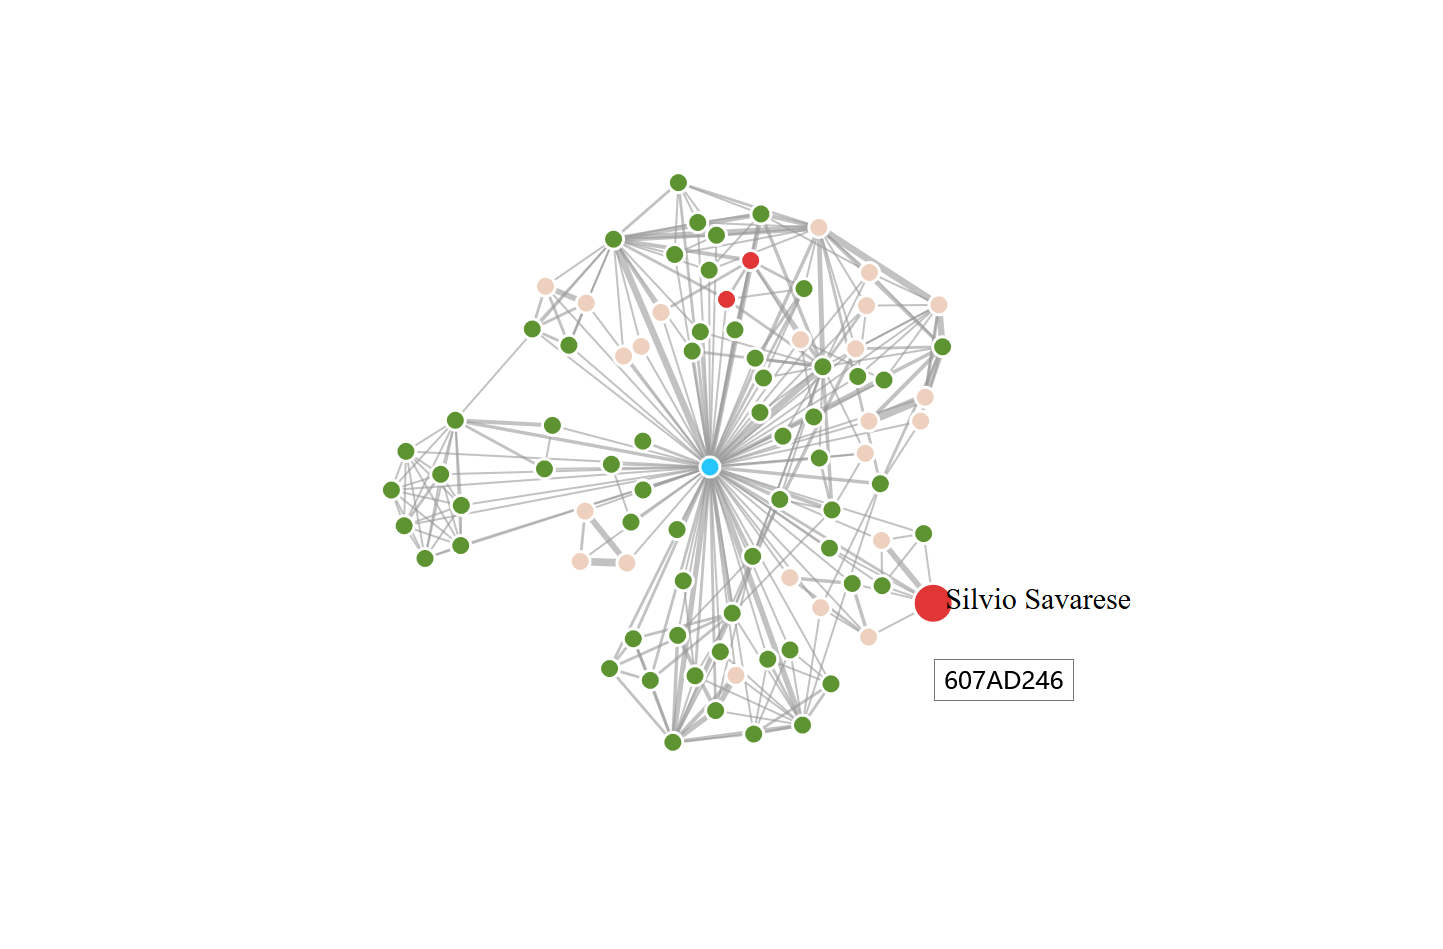
\includegraphics[width=.8\textwidth]{img/graph.png}
\caption{Force-Directed Graph}
\end{figure}
The blue, red, green and beige nodes represent the author himself/herself, his/her instructors, his/her students and other collaborators. So the graph is quite intutive, as an author is very likely to have many students and only a few instructors.
    \newpage
    \section{Conclusion and Prospect}
Doing this project really takes me a lot of time but equips me with plenty of skiils in return. 

I have learned the basic usage of Javascript, jQuery and D3.js. Though my understanding of them is not very deep now, I do feel that they are useful and powerful. So I think I will further my learning of them in the future.

More importantly, after learning MVC in Lab 2, I have gained some insight into front-end and back-end seperation this time. 
\end{document}
